%%%%%%%%%%%%%%%%%%%%%%%%%%%%%%%%%%%%%%%%%
% Article EcoFoG
% Version 2.1 (23/10/2017)
%
% adapté de :
% Stylish Article
% LaTeX Template
% Version 1.0 (31/1/13)
%
% This template has been downloaded from:
% http://www.LaTeXTemplates.com
%
% Original author:
% Mathias Legrand (legrand.mathias@gmail.com)
%
% License:
% CC BY-NC-SA 3.0 (http://creativecommons.org/licenses/by-nc-sa/3.0/)
%
%%%%%%%%%%%%%%%%%%%%%%%%%%%%%%%%%%%%%%%%%


%----------------------------------------------------------------------------------------
%	PACKAGES AND OTHER DOCUMENT CONFIGURATIONS
%----------------------------------------------------------------------------------------

\documentclass[fleqn,10pt]{ArtEcoFoG} % Document font size and equations flushed left

\setcounter{tocdepth}{3} % Show only three levels in the table of contents section: sections, subsections and subsubsections


% Pandoc environments
\usepackage{framed}
\usepackage{fancyvrb}
\providecommand{\tightlist}{%
  \setlength{\itemsep}{0pt}\setlength{\parskip}{0pt}}
\newcommand{\VerbBar}{|}
\newcommand{\VERB}{\Verb[commandchars=\\\{\}]}
\DefineVerbatimEnvironment{Highlighting}{Verbatim}{commandchars=\\\{\}, fontsize=\scriptsize} % Code R
\definecolor{shadecolor}{RGB}{248,248,248}
\newenvironment{Shaded}{\begin{snugshade}}{\end{snugshade}}
\newcommand{\KeywordTok}[1]{\textcolor[rgb]{0.13,0.29,0.53}{\textbf{{#1}}}}
\newcommand{\DataTypeTok}[1]{\textcolor[rgb]{0.13,0.29,0.53}{{#1}}}
\newcommand{\DecValTok}[1]{\textcolor[rgb]{0.00,0.00,0.81}{{#1}}}
\newcommand{\BaseNTok}[1]{\textcolor[rgb]{0.00,0.00,0.81}{{#1}}}
\newcommand{\FloatTok}[1]{\textcolor[rgb]{0.00,0.00,0.81}{{#1}}}
\newcommand{\ConstantTok}[1]{\textcolor[rgb]{0.00,0.00,0.00}{{#1}}}
\newcommand{\CharTok}[1]{\textcolor[rgb]{0.31,0.60,0.02}{{#1}}}
\newcommand{\SpecialCharTok}[1]{\textcolor[rgb]{0.00,0.00,0.00}{{#1}}}
\newcommand{\StringTok}[1]{\textcolor[rgb]{0.31,0.60,0.02}{{#1}}}
\newcommand{\VerbatimStringTok}[1]{\textcolor[rgb]{0.31,0.60,0.02}{{#1}}}
\newcommand{\SpecialStringTok}[1]{\textcolor[rgb]{0.31,0.60,0.02}{{#1}}}
\newcommand{\ImportTok}[1]{{#1}}
\newcommand{\CommentTok}[1]{\textcolor[rgb]{0.56,0.35,0.01}{\textit{{#1}}}}
\newcommand{\DocumentationTok}[1]{\textcolor[rgb]{0.56,0.35,0.01}{\textbf{\textit{{#1}}}}}
\newcommand{\AnnotationTok}[1]{\textcolor[rgb]{0.56,0.35,0.01}{\textbf{\textit{{#1}}}}}
\newcommand{\CommentVarTok}[1]{\textcolor[rgb]{0.56,0.35,0.01}{\textbf{\textit{{#1}}}}}
\newcommand{\OtherTok}[1]{\textcolor[rgb]{0.56,0.35,0.01}{{#1}}}
\newcommand{\FunctionTok}[1]{\textcolor[rgb]{0.00,0.00,0.00}{{#1}}}
\newcommand{\VariableTok}[1]{\textcolor[rgb]{0.00,0.00,0.00}{{#1}}}
\newcommand{\ControlFlowTok}[1]{\textcolor[rgb]{0.13,0.29,0.53}{\textbf{{#1}}}}
\newcommand{\OperatorTok}[1]{\textcolor[rgb]{0.81,0.36,0.00}{\textbf{{#1}}}}
\newcommand{\BuiltInTok}[1]{{#1}}
\newcommand{\ExtensionTok}[1]{{#1}}
\newcommand{\PreprocessorTok}[1]{\textcolor[rgb]{0.56,0.35,0.01}{\textit{{#1}}}}
\newcommand{\AttributeTok}[1]{\textcolor[rgb]{0.77,0.63,0.00}{{#1}}}
\newcommand{\RegionMarkerTok}[1]{{#1}}
\newcommand{\InformationTok}[1]{\textcolor[rgb]{0.56,0.35,0.01}{\textbf{\textit{{#1}}}}}
\newcommand{\WarningTok}[1]{\textcolor[rgb]{0.56,0.35,0.01}{\textbf{\textit{{#1}}}}}
\newcommand{\AlertTok}[1]{\textcolor[rgb]{0.94,0.16,0.16}{{#1}}}
\newcommand{\ErrorTok}[1]{\textcolor[rgb]{0.64,0.00,0.00}{\textbf{{#1}}}}
\newcommand{\NormalTok}[1]{{#1}}
\usepackage{longtable,booktabs}
\usepackage{caption}
% These lines are needed to make table captions work with longtable:
\makeatletter
\def\fnum@table{\tablename~\thetable}
\makeatother
% longtable 2 columns
% https://tex.stackexchange.com/questions/161431/how-to-solve-longtable-is-not-in-1-column-mode-error
\makeatletter
\let\oldlt\longtable
\let\endoldlt\endlongtable
\def\longtable{\@ifnextchar[\longtable@i \longtable@ii}
\def\longtable@i[#1]{\begin{figure}[t]
\onecolumn
\begin{minipage}{0.5\textwidth}\scriptsize
\oldlt[#1]
}
\def\longtable@ii{\begin{figure}[t]
\onecolumn
\begin{minipage}{0.5\textwidth}\scriptsize
\oldlt
}
\def\endlongtable{\endoldlt
\end{minipage}
\twocolumn
\end{figure}}
\makeatother

\usepackage{graphicx,grffile}
\makeatletter
\def\maxwidth{\ifdim\Gin@nat@width>\linewidth\linewidth\else\Gin@nat@width\fi}
\def\maxheight{\ifdim\Gin@nat@height>\textheight0.8\textheight\else\Gin@nat@height\fi}
\makeatother
% Scale images if necessary, so that they will not overflow the page
% margins by default, and it is still possible to overwrite the defaults
% using explicit options in \includegraphics[width, height, ...]{}
\setkeys{Gin}{width=\maxwidth,height=\maxheight,keepaspectratio}

% User-adder preamble
\usepackage{amsmath}

%----------------------------------------------------------------------------------------
%	ARTICLE INFORMATION
%----------------------------------------------------------------------------------------

\JournalInfo{Hal 00679993} % Journal information
\Archive{DOI xxxx} % Additional notes (e.g. copyright, DOI, review/research article)

\PaperTitle{Titre de l'article} % Article title

\Authors{
Prénom Nom\textsuperscript{1*}\\ Deuxième Auteur\textsuperscript{2}
} % Authors
\affiliation{
\textsuperscript{1}UMR EcoFoG, AgroParistech, CNRS, Cirad, INRA, Université des Antilles,
Université de Guyane.\\ \hspace{1em} Campus Agronomique, 97310 Kourou, France.\\\textsuperscript{2}Department of Ecology, University of Edimburgh\\ \hspace{1em} Street address, Zip code, Country.
}
\affiliation{*\textbf{Contact}: prenom.nom@ecofog.gf, http://www.ecofog.gf/spip.php?article47} % Corresponding author

\Keywords{mot-clés, séparés par des virgules} % Keywords - if you don't want any simply remove all the text between the curly brackets
\newcommand{\keywordname}{Mots-clés} % Defines the keywords heading name

%----------------------------------------------------------------------------------------
%	ABSTRACT
%----------------------------------------------------------------------------------------

\Abstract{
Résumé de l'article.
}

%----------------------------------------------------------------------------------------

\begin{document}

\selectlanguage{french}

\flushbottom % Makes all text pages the same height

\maketitle % Print the title and abstract box

\tableofcontents % Print the contents section

\thispagestyle{empty} % Removes page numbering from the first page

%----------------------------------------------------------------------------------------
%	ARTICLE CONTENTS
%----------------------------------------------------------------------------------------


\section{Introduction}\label{introduction}

Ce modèle permet la rédaction d'articles au format Markdown. Il produit
directement des articles bien formatés pour l'auto-archivage (dépôt sur
HAL par exemple) ou sous d'autres formats, par exemple HTML.

\section{R Markdown}\label{markdown}

Markdown est un langage très simple pour produire divers types de
documents: HTML, PDF, et Word entre autres. Sa documentation est
disponible sur le site de RStudio\footnote{https://github.com/citation-style-language/styles}.

Markdown est étendu par Bookdown \footnote{\url{https://bookdown.org/yihui/bookdown/}},
qui permet la rédaction de livres et une syntaxe plus efficace pour les
articles. Ce document est réalisé avec Markdown dans RStudio: knitr
traite le code Markdown, le passe à Pandoc pour sa transformaton en
Latex, enfin MikteX le compile en PDF.

\subsection{Intérêt}\label{interet}

Markdown est très simple à apprendre.

Markdown permet d'intégrer son code R pour un résultat
\emph{reproductible}.

Markdown permet de produire, sans réécrire le texte, un document dans
différents formats: article Latex ou Word par exemple.

\subsection{Comment faire}\label{comment-faire}

Dans RStudio, créer un nouveau document de type Document R Markdown.
L'assistant permet de choisir entre divers formats. Les plus
intéressants sont:

\begin{figure}
\centering
\includegraphics{NouveauRMarkdown.PNG}
\caption{\label{fig:nouveau}Nouveau document}
\end{figure}

\begin{itemize}
\item
  Document: rapport simple
\item
  Presentation: diaporama
\item
  From template: à partir de modèles installés par des packages. Les
  modèles du package EcoFoG sont affichés (voir figure
  \ref{fig:nouveau}): choisir Article EcoFoG.
\item
  Ecrire le document dans RStudio.
\item
  Cliquer sur le bouton \textbf{Knit} de RStudio génère le document au
  format demandé.
\end{itemize}

\section{Code}\label{code}

Les principales caractéristiques de Markdown sont résumées ici.

\subsection{Code R}\label{code-r}

Le code R est inclus dans des bouts de code (\emph{code chunks}):

\begin{Shaded}
\begin{Highlighting}[]
\KeywordTok{head}\NormalTok{(cars)}
\end{Highlighting}
\end{Shaded}

\begin{verbatim}
##   speed dist
## 1     4    2
## 2     4   10
## 3     7    4
## 4     7   22
## 5     8   16
## 6     9   10
\end{verbatim}

\subsection{Tableaux}\label{tableaux}

Les séparateurs horizontaux - et verticaux \textbar{} permettent de
dessiner un tableau. Les tableaux peuvent aussi être produits par du
code R, avec le package knitr:

\begin{Shaded}
\begin{Highlighting}[]
\KeywordTok{names}\NormalTok{(iris) <-}\StringTok{ }\KeywordTok{c}\NormalTok{(}\StringTok{"Longueur sépales"}\NormalTok{, }\StringTok{"Largeur"}\NormalTok{, }\StringTok{"Longueur pétales"}\NormalTok{, }\StringTok{"Largeur"}\NormalTok{, }\StringTok{"Espèce"}\NormalTok{)}
\NormalTok{knitr}\OperatorTok{::}\KeywordTok{kable}\NormalTok{(}\KeywordTok{head}\NormalTok{(iris), }\DataTypeTok{caption=}\StringTok{"Tableau créé par R"}\NormalTok{, }\DataTypeTok{longtable =} \OtherTok{TRUE}\NormalTok{, }\DataTypeTok{booktabs =} \OtherTok{TRUE}\NormalTok{)}
\end{Highlighting}
\end{Shaded}

\begin{longtable}[t]{rrrrl}
\caption{\label{tab:kable}Tableau créé par R}\\
\toprule
Longueur sépales & Largeur & Longueur pétales & Largeur & Espèce\\
\midrule
5.1 & 3.5 & 1.4 & 0.2 & setosa\\
4.9 & 3.0 & 1.4 & 0.2 & setosa\\
4.7 & 3.2 & 1.3 & 0.2 & setosa\\
4.6 & 3.1 & 1.5 & 0.2 & setosa\\
5.0 & 3.6 & 1.4 & 0.2 & setosa\\
5.4 & 3.9 & 1.7 & 0.4 & setosa\\
\bottomrule
\end{longtable}

Une légende est possible et le référencement aussi (tableau
\ref{tab:kable}). Attention, la largeur des tableaux est limitée à une
colonne de texte, et les retours à la ligne dans les cellules ne sont
pas pris en charge.

\subsection{Figures}\label{figures}

\begin{Shaded}
\begin{Highlighting}[]
\KeywordTok{plot}\NormalTok{(pressure)}
\end{Highlighting}
\end{Shaded}

\begin{figure}
\centering
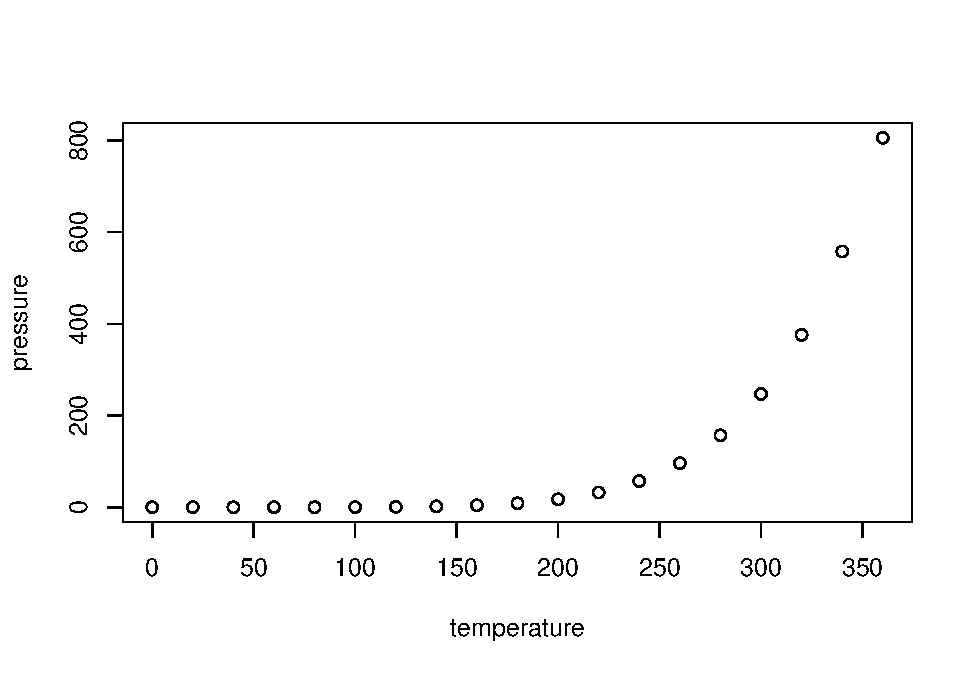
\includegraphics{Saucisson_files/figure-latex/pressure-1.pdf}
\caption{\label{fig:pressure}Titre de la figure}
\end{figure}

Les figures peuvent être créées par le code R (figure
\ref{fig:pressure}). Avec Bookdown, une étiquette est associée à chaque
figure: son nom est \texttt{fig:xxx} où \texttt{xxx} est le nom du bout
de code R. Les renvois se fonct avec la commande
\texttt{\textbackslash{}@ref(fig:xxx)}.

Une figure peut utiliser toute la largeur de la page en ajoutant les
options suivantes dans l'entête du bout de code qui la génère:
\texttt{fig.env="figure*"}et \texttt{out.extra=""}.

Les figures existantes sont intégrées dans un bout de code par la
fonction \texttt{include\_graphics}, voir la figure \ref{fig:nouveau}.

\subsection{Listes}\label{listes}

Les listes sont indiquées par des *, + et - (trois niveaux
hiérarchiques) ou des nombres 1., i. et A. (listes numérotées).

\begin{itemize}
\item
  Liste

  \begin{itemize}
  \tightlist
  \item
    sous-liste
  \end{itemize}
\item
  deuxième élément
\item
  Suite de la liste
\end{itemize}

\subsection{Maths}\label{maths}

Les équations au format Latex peuvent être insérées en ligne, comme
\(A=\pi r^2\) ou isolées comme \[e^{i \pi} = -1.\]

Elles peuvent être numérotées (voir équation \eqref{eq:disque}) en
utlisant l'environnement \emph{equation} :

\begin{equation}
A = \pi r^2.
\label{eq:disque}
\end{equation}

\subsection{Références croisées}\label{references-croisees}

Les figures et tableaux ont une étiquette générée automatiquement,
identique au nom du bout de code préfixé par \texttt{fig:} et
\texttt{tab:}.

Pour les équations, l'étiquette est ajoutée manuellement par le code
\texttt{(\textbackslash{}\#eq:xxx)} avant la fin de l'équation.

Les sections peuvent recevoir une étiquette en terminant leur titre par
\texttt{\{\#yyy\}}.

Des signets peuvent aussi être placés librement dans le texte avec la
commande \texttt{(ref:zzz)}.

Dans tous les cas, l'appel à la référence est fait par la commande
\texttt{\textbackslash{}@ref(ref:zzz)}.

\subsection{Bibliographie}\label{bibliographie}

Les références bibliographiques incluses dans le fichier references.bib
peuvent être appelées dans le texte, entre parenthèses
\citep{Marcon2014c}, ou dans le texte, à la façon de
\citet{Marcon2014c}.

La bibliographie est traitée par Pandoc lors de la production de
documents Word ou HTML. Le sytle bibliographique peut être précisé, en
ajoutant la ligne

\begin{verbatim}
csl:nom_du_fichier.csl
\end{verbatim}

dans l'entête du document et en copiant le fichier de style \emph{.csl}
dans le dossier du projet. Plus d'un millier de styles sont disponibles
\footnote{https://github.com/citation-style-language/styles}.

Pour les documents PDF, la bibliographie est gérée par \LaTeX: c'est
pourquoi l'extension \emph{.bib} du fichier doit être supprimée dans la
déclaration de la base bibliographique. Le style est inclus dans le
modèle EcoFoG: c'est celui de \emph{Methods in Ecology and Evolution}.
Il ne peut pas être changé, pour assurer l'homogénéité des documents
produits.

Pour préparer la soumission d'un manuscrit à une revue, il faudra ouvrir
le fichier \emph{.tex} intermédiaire produit par Pandoc et copier le
contenu de l'environnement \{document\} dans le modèle proposé par la
revue, qui se chargera du formatage.

\section{Types de document}\label{types-de-document}

Ce modèle est prévu pour fonctionner avec le modèle Article d'EcoFoG en
LaTeX et produire des documents au format PDF. En changeant l'entête du
document, un fichier HTML est produit: décommenter

\begin{verbatim}
 bookdown::gitbook
\end{verbatim}

et commenter

\begin{verbatim}
bookdown::pdf_book:
\end{verbatim}

et les deux lignes suivantes qui en dépendent; compléter le nom du
fichier \emph{.bib} avec son extension sur la ligne
\texttt{bibliography} (LaTeX attend le nom du fichier sans extension
contrairement aux autres générateurs).

Pour produire un document Word, procéder de la même façon que pour un
fichier HTML en décommentant

\begin{verbatim}
bookdown::word_document2.
\end{verbatim}

Le document Word peut ensuite être modifié pour respecter les
instructions aux auteurs des revues : double interlignage, police, etc.

\subsection{Document HTML/PDF}\label{document-htmlpdf}

Pour un usage quotidien: le modèle HTML simple à utiliser, son format de
sortie est propre correct. Le résultat est bien plus clair que du code R
commenté.

\subsection{Document Word}\label{document-word}

Son contenu peut être mis en forme ou copié dans un modèle. Les styles
de texte standard sont ``First Paragraph'' et ``Corps de de texte''.

L'intérêt du format Word est de produire un manuscrit pour les revues
qui ne supportent pas \LaTeX. Le style bibliographique de la revue est
très probablement disponible au format \emph{.csl}, ce qui permet de
minimiser la préparation manuelle.

\subsection{Présentation Beamer}\label{presentation-beamer}

Utiliser le modèle \emph{Présentation EcoFoG} proposé par le package.

Le document produit est un diaporama Beamer respectant la charte
graphique 2018.

\subsection{Autres Modèles}\label{autres-modeles}

Le package rticle fournit des modèles d'articles (PLOS, PNAS, etc.). Le
package xaringan fournit un modèle de présentation HTML 5.

Le modèle Ouvrage du package EcoFoG permet d'écrire des livres.

La dernière ligne du modèle (bout de code R) doit être conservée pour
afficher le titre \emph{References} (à traduire éventuellement dans la
langue du document) au format HTML. Le titre de niveau 1
\emph{Références} doit être ajouté manuellement aux fichiers Word.

%----------------------------------------------------------------------------------------
%	REFERENCE LIST
%----------------------------------------------------------------------------------------

\bibliographystyle{mee}
\bibliography{references}

%----------------------------------------------------------------------------------------

\end{document}
